\chapter{Resultat}
\textit{I dette kapitel beskrives resultatet for evaluering af systemets anvendelighed i forhold til at besvare problemformuleringen. I denne forbindelse er systemets anvendelighed vurderet og testet ved kvantitative og kvalitative metoder.}

\section{Systemets anvendelighed}
Til evaluering af systemet til risikovurdering af lægemiddelskift var der repræsenteret 11 medarbejdere fordelt på forskellige afdelinger fra SRN, 8 fra Lægemiddelinformation, 2 fra Medicinservice og 1 fra Klinisk Farmaci. Resultatet af systemet til risikovurdering er opdelt i forhold til at teste sammenhængen mellem risikovurderingerne foretaget af systemet og medarbejderne fra SRN. Derudover vurderes risikoscore samt risikofaktorer og deres vægtning.

\subsection{Sammenligning af risikovurderinger}
Vurderingerne foretaget af medarbejdere fra SRN er sammenholdt i forhold til at definere en Golden Standard. Denne er bestemt ud fra at over 60~\% af medarbejderne var enige i om lægemiddelskiftet krævede uddybende information. Dette er gjort for at sammenligne Golden Standard, medarbejdernes vurdering, med Lægemiddel Nyt i forhold til at undersøge systemts sensitivitet og specificitet. Vurderingerne af lægemiddelskift fremgår af Tabel \ref{table:test1}, hvor de individuelle vurderinger af medarbejderne fremgår af Tabel \ref{table:resultat} i Appendiks \ref{App:Resultat}.

\begin{table}[H]
\caption{Sammenligning af vurderinger fra henholdsvis Lægemiddel Nyt og Golden Standard bestemt ud vurderinger fra medarbejderne i forhold til uddybende information. Uenighed mellem disse er markeret med gul, mens en vurdering under 60~\% enighed mellem medarbejderne er markeret med rød.}
\vspace{2mm}
\label{table:test1}
\centering
\begin{tabular}{l|c|c|c|c|c|c|c|c|c|c|c|c|c|c|c|c|c}
\rowcolor[HTML]{C0C0C0} \textbf{} & \multicolumn{11}{|c}{\textbf{Lægemiddelskift nummer}} \\
\rowcolor[HTML]{C0C0C0} & \textbf{1} & \textbf{2} & \textbf{3} & \textbf{4} & \textbf{5} & \textbf{6} & \textbf{7} &  \textbf{8} & \textbf{9} & \textbf{10} & \textbf{11}   \\ \hline
%\textbf{Risikoscore} & 0 & 0 & 5 & 5 & 5 & 5 & 5 & 5 & 10 & 10 & 10  \\ \hline
\textbf{Lægemiddel Nyt} & nej & nej & nej & nej & nej & nej & nej & nej & ja &\cellcolor[HTML]{F6F6C3} ja & nej \\ \hline
\textbf{Golden Standard} & nej & nej & nej& nej & nej &nej & nej & nej& ja & \cellcolor[HTML]{F6F6C3}nej & nej \\ \hline
\rowcolor[HTML]{C0C0C0} & \multicolumn{11}{|c}{\textbf{Lægemiddelskift nummer}} \\
\rowcolor[HTML]{C0C0C0} & \textbf{12} & \textbf{13} & \textbf{14} &  \textbf{15} & \textbf{16} & \textbf{17} & \textbf{18} & \textbf{19} & \textbf{20} & \textbf{21} & \textbf{22}  \\ \hline
%\textbf{Risikoscore} & 15 & 15 & 15 & 15 & 20 & 20 & 20 & 25 & 25 & 25 & 30 \\ \hline
\textbf{Lægemiddel Nyt} & nej & nej & \cellcolor[HTML]{F6F6C3}nej & nej & nej & nej & \cellcolor[HTML]{F6F6C3}ja & \cellcolor[HTML]{F6F6C3}nej & \cellcolor[HTML]{F6F6C3}ja & \cellcolor[HTML]{F6F6C3}nej & \cellcolor[HTML]{F6F6C3}nej\\ \hline
\textbf{Golden Standard} & \cellcolor[HTML]{F6E6E5} - & nej & \cellcolor[HTML]{F6F6C3}ja & nej & nej & nej & \cellcolor[HTML]{F6F6C3}nej & \cellcolor[HTML]{F6F6C3}ja & \cellcolor[HTML]{F6F6C3}nej & \cellcolor[HTML]{F6F6C3}ja & \cellcolor[HTML]{F6F6C3}ja \\ \hline
\rowcolor[HTML]{C0C0C0} & \multicolumn{11}{|c}{\textbf{Lægemiddelskift nummer}} \\ 
\rowcolor[HTML]{C0C0C0} & \textbf{23} & \textbf{24} & \textbf{25} & \textbf{26} & \textbf{27} & \textbf{28} &  \textbf{29} & \textbf{30} & \textbf{31} & \textbf{32} & \textbf{33}  \\ \cline{1-10}
\textbf{Lægemiddel Nyt} & nej & \cellcolor[HTML]{F6F6C3}ja & nej & nej & nej & ja & ja & ja & ja & \cellcolor[HTML]{F6F6C3}nej & ja\\ \hline
\textbf{Golden Standard} & nej & \cellcolor[HTML]{F6F6C3}nej & nej & nej & nej & ja & ja& ja & ja& \cellcolor[HTML]{F6F6C3}ja & ja \\\hline
\end{tabular}
\end{table}

Det fremgår af Tabel \ref{table:test1} at der ikke er en 60~\% enighed mellem medarbejderne i forhold til lægemiddelskift nummer 12, hvorfor dette lægemiddelskift undlades i den efterfølgende databehandling. Derudover fremgår det at der er uenighed mellem Lægemiddel Nyt og medarbejdernes vurdering for 9 lægemiddelskift svarende til 27~\% og enighed for 23, svarende til 69,7~\%. For at undersøge systemets nøjagtighed beregnes sensitivitet og specificitet, hvilket fremgår af Tabel \ref{table:PositivNegativ}.

\begin{table}[H]
\caption{Krydstabel for Lægemiddel Nyt og Golden Standard. Sensitiviteten er markeret med blå og specificiteten er angivet med grøn.}
\vspace{2mm}
\label{table:PositivNegativ}
\centering
\begin{tabular}{ll|l|l|l|l}
 \rowcolor[HTML]{C0C0C0}                          &                          &                            & \multicolumn{2}{c|}{\textbf{Golden Standard}} &        \\ 
  \rowcolor[HTML]{C0C0C0}                                                         &                          &                            & Positiv       & Negativ          & Antal  \\ \hline
\cellcolor[HTML]{C0C0C0} \textbf{Lægemiddel}                                                \hspace{-0.5cm} \multirow{4}{*}{} &  \cellcolor[HTML]{C0C0C0}                                                      Positiv \multirow{2}{*}{} & Antal & 6                & 4                & 10     \\ \cline{3-6} 
\cellcolor[HTML]{C0C0C0}                                                                \textbf{Nyt} &   \cellcolor[HTML]{C0C0C0}                                               & \% indenfor Golden Standard & \cellcolor[HTML]{ECF4FF} 54,5 \%           & 19,0 \%           & 31,3 \% \\\cline{2-6}
\cellcolor[HTML]{C0C0C0}                                                                                 & \cellcolor[HTML]{C0C0C0}                                                                               Negativ \multirow{2}{*}{} & Talte & 5                & 17               & 22     \\ \cline{3-6}
          \cellcolor[HTML]{C0C0C0}                                                                             &                         \cellcolor[HTML]{C0C0C0}                                                        & \% indenfor Golden Standard & 45,5 \%           & \cellcolor[HTML]{D4EED3}81,0 \%            & 68,8 \% \\ \hline
 \cellcolor[HTML]{C0C0C0}                                                                            \textbf{Total}                         &                          \cellcolor[HTML]{C0C0C0}                                                                             & Antal                     & 11               & 21               & 32     \\ \cline{3-6}
                          \cellcolor[HTML]{C0C0C0}                                                                                   &                           \cellcolor[HTML]{C0C0C0}                                                                            & \% indenfor Golden Standard & 100 \%            & 100\%            & 100 \% 
\end{tabular}
\end{table}

Af Tabel \ref{table:PositivNegativ} fremgår det at lægemiddelskiftet blev vurderet positiv, hvilket vil sige at det krævende uddybende information, for både Lægemiddel Nyt og medarbejderne i 6 tilfælde. Modsat blev det i 21 tilfælde vurderet negativt af både Lægemiddel Nyt og medarbejderne, hvilket vil sige at lægemiddelskiftet ikke krævede uddybende informationer. Lægemiddelskiftet blev i 5 tilfælde vurderet negativt af Lægemiddel Nyt og positivt af medarbejderne, mens det i 4 tilfælde blev vurderet positivt af Lægemiddel Nyt, men negativt af medarbejderne. 

Ud fra Tabel \ref{table:PositivNegativ} fremgår det ligeledes at systemets sensitivitet er 54,5~\% og sensitivitet er 81~\%.  Dette vil sige, at systemet i 54,5~\% af tilfældene vil foretage en korrekt vurdering af om lægemiddelskift kræver uddybende information og i 81~\% af tilfældene vil foretage en korrekt vurdering af om lægemiddelskiftet ikke kræver uddybende information. Derudover vil systemt i 45,5~\% af tilfældene give anledning til type 2 error, hvilket vil sige at systemet vil vurdere at et lægemiddelskift ikke kræver uddybende information, hvor dette var tilfældet. Yderligere vil systemet i 19~\% af tilfældene give anledning til type 1 error, hvor systemet vil vurdere at et lægemiddelskift som ikke kræver uddybende information vil blive vurderet til at kræve dette.

\subsection{Vurdering af risikoscore}
Til at evaluere risikoscore og vægtningen af disse sammenlignes vurderingerne foretaget af medarbejderne ved Golden Standard og risikoscore udregnet af systemet, som fremgår af Tabel \ref{table:test2}.

\begin{table}[H]
\caption{Risikoscore og vurdering af lægemiddelskift angivet som Golden Standard for medarbejderne. Vurdering under 60~\% enighed mellem medarbejderne er markeret med rød.}
\vspace{2mm}
\label{table:test2}
\centering
\begin{tabular}{l|c|c|c|c|c|c|c|c|c|c|c|c|c|c|c|c|c}
\rowcolor[HTML]{C0C0C0} \textbf{} & \multicolumn{11}{|c}{\textbf{Lægemiddelskift nummer}} \\
\rowcolor[HTML]{C0C0C0} & \textbf{1} & \textbf{2} & \textbf{3} & \textbf{4} & \textbf{5} & \textbf{6} & \textbf{7} &  \textbf{8} & \textbf{9} & \textbf{10} & \textbf{11}   \\ \hline
\textbf{Risikoscore} & 0 & 0 & 5 & 5 & 5 & 5 & 5 & 5 & 10 & 10 & 10  \\ \hline
%\textbf{Lægemiddel Nyt} & nej & nej & nej & nej & nej & nej & nej & nej & ja &\cellcolor[HTML]{F6F6C3} ja & nej \\ \hline
\textbf{Golden Standard} & nej & nej & nej& nej & nej &nej & nej & nej& ja & nej & nej \\ \hline
\rowcolor[HTML]{C0C0C0} & \multicolumn{11}{|c}{\textbf{Lægemiddelskift nummer}} \\
\rowcolor[HTML]{C0C0C0} & \textbf{12} & \textbf{13} & \textbf{14} &  \textbf{15} & \textbf{16} & \textbf{17} & \textbf{18} & \textbf{19} & \textbf{20} & \textbf{21} & \textbf{22}  \\ \hline
\textbf{Risikoscore} & \cellcolor[HTML]{F6E6E5} 15 & 15 & 15 & 15 & 20 & 20 & 20 & 25 & 25 & 25 & 30 \\ \hline
%\textbf{Lægemiddel Nyt} & nej & nej & \cellcolor[HTML]{F6F6C3}nej & nej & nej & nej & \cellcolor[HTML]{F6F6C3}ja & \cellcolor[HTML]{F6F6C3}nej & \cellcolor[HTML]{F6F6C3}ja & \cellcolor[HTML]{F6F6C3}nej & \cellcolor[HTML]{F6F6C3}nej\\ \hline
\textbf{Golden Standard} & \cellcolor[HTML]{F6E6E5} - & nej & ja & nej & nej & nej & nej & ja & nej & ja & ja \\ \hline
\rowcolor[HTML]{C0C0C0} & \multicolumn{11}{|c}{\textbf{Lægemiddelskift nummer}} \\ 
\rowcolor[HTML]{C0C0C0} & \textbf{23} & \textbf{24} & \textbf{25} & \textbf{26} & \textbf{27} & \textbf{28} &  \textbf{29} & \textbf{30} & \textbf{31} & \textbf{32} & \textbf{33}  \\ \cline{1-10}
\textbf{Risikoscore} & 30 & 30 & 35 & 35 & 35 & 40 & 40 & 45 & 50 & 50 & 55 \\ \hline 
%\textbf{Lægemiddel Nyt} & nej & \cellcolor[HTML]{F6F6C3}ja & nej & nej & nej & ja & ja & ja & ja & \cellcolor[HTML]{F6F6C3}nej & ja\\ \hline
\textbf{Golden Standard} & nej & nej & nej & nej & nej & ja & ja& ja & ja&ja & ja \\\hline
\end{tabular}
\end{table}

Ud fra Tabel \ref{table:test2} fremgår det at lægemiddelskift med en risikoscore på 10, 15, 25 og 30 er vurderet forskelligt i forhold til uddybende information. Derudover fremgår det at der ved lægemiddelskift nummer 12 var under 60~\% enighed mellem medarbejderne, hvormed dette skift ikke tages med i videre behandling. Sensitiviteten og specificiteten er illustreret via Figur \ref{fig:ROC1}. 

\vspace{-0.5cm}
\begin{figure}[H]\centering
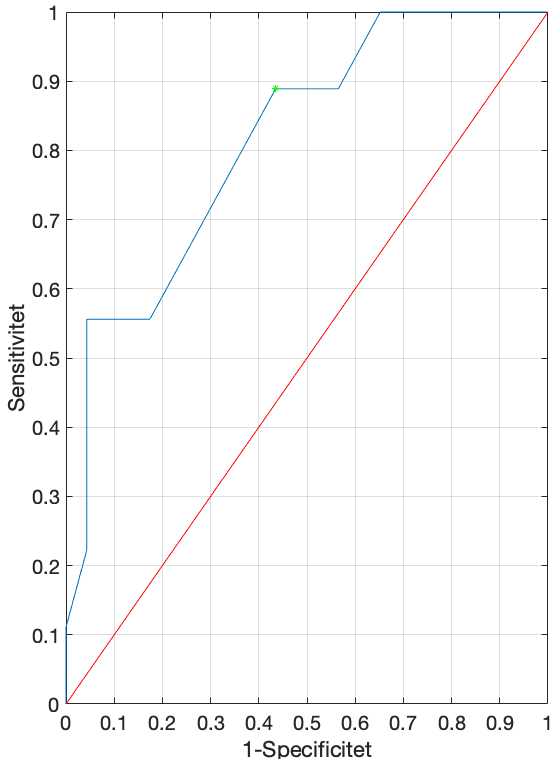
\includegraphics[width=0.7\textwidth]{billeder/ROC.png} 
	\caption{ROC-kurve. På y-aksen er sensitivitet angivet og x-aksen 1-specificitet. Den røde linje indikerer reference og den blå linje ROC-kurven.}
	\label{fig:ROC1}  
\end{figure}

På Figur \ref{fig:ROC1} fremgår det at ROC-kurven, som er illustreret af den blå linje, er over reference linjen, som er illustreret af den røde, hvilket indikerer, at det er et god redskab til risikovurdering, hvilket understøttes af test for arealet under kurven som fremgår af Tabel \ref{table:AUC}.

\begin{table}[H]
\caption{Areal under kurven}
\vspace{2mm}
\label{table:AUC}
\centering
\begin{tabular}{l|l|l|l|l}
 \rowcolor[HTML]{C0C0C0}   &                         & \textbf{Signifikant} &
 \multicolumn{2}{c}{\textbf{95 \% Konfidensinterval}}  \\ 
  \rowcolor[HTML]{C0C0C0}                                                         \textbf{Areal} &  \textbf{Standard error}                       &  & Nedre grænse      & Øvre grænse    \\
%0,766 & 0,090 & 0,017 & 0,589 & 0,942  \\
0,840 & 0,074 & 0,002 & 0,696 & 0,984 \\
\end{tabular}
\end{table}

Af Tabel \ref{table:AUC} fremgår det at arealet under kurven er 0,840, hvilket vil sige at systemet er god, givet at en værdi på 1 antager at systemets vurderingen er perfekt. Derudover det det angivet at resultat er  statistisk signifikant (p=0,002) og har en nedre grænse på 0,696 og øvre grænse på 0,984 ved et 95~\% konfidensinterval.

%Determine cut-off score -> svære at bedømme -> blancere sensitivitet med specificitet. Afhænger af applikationen, kan måske tollere høj sensitivitet og lav specificitet eller omvendt. Det er ud fra denne man kan bestemme cut-off score for det redskab man anvender. 

%cut-of 88.5 \% af de positive outcome vil være korrekt identificeret, og 29, 4 ~\% af de negative vil være incorrect identificeret som positiv (falsk positiv)

\subsection{Vurdering af risikofaktorer og vægtning}

 





%\section{Systemets performance}
%Ud af lægemiddelskiftene var der for 13 lægemidler enighed mellem medarbejderne fra SRN. Ud af 33 blev 11 lægemidler vurderet til ikke at krævede uddybende samt at 2 lægemidler krævede uddybende information ved implementering af disse i klinikken. Størstedelen af lægemiddelskift blev vurderet af 9 ud af 11 til ikke at kræve uddybende information, mens 2 medarbejdere vurderede at størstedelen af lægemidlerne krævede uddybende information, hvilket er markeret med blåt i Tabel \ref{table:test1}. Gennemsnittet blev vurderet til at 12,27 lægemidler, svarende til 37,19~\%, krævede uddybende information, mens 20,63 lægemidler, svarende til 62,5~\%, ikke krævede uddybende information, hvilket ligeledes fremgår af Tabel \ref{table:test1}. 

%\begin{table}[H]
%\caption{Krydstabel for vurderingen ja eller nej i forhold til uddybende information om lægemiddelskiftet og testpersoner samt lægemiddel Nyt, som er indikeret som nummer 12. \textcolor{red}{Er i tvivl, hvorvidt det giver mening at have lægemiddel Nyt med i denne test}}
%\vspace{2mm}
%\label{table:test1}
%\centering
%\begin{tabular}{l|c|c|c|c|c|c|c|c|c|c|c|c|c}
%\rowcolor[HTML]{C0C0C0}
% & \multicolumn{11}{|c|}{\textbf{Testperson}} & \textbf{} & \textbf{Total}    \\
%\rowcolor[HTML]{C0C0C0}  & \textbf{1}  & \textbf{2}  & \textbf{3} & \textbf{4} & \textbf{5} & \textbf{6} & \textbf{7} & \textbf{8} & \textbf{9} & \textbf{10} & \textbf{11} & \textbf{12}  & \\ 
%\cellcolor[HTML]{C0C0C0}{Antal af Nej}            & 24 & 20 & 21  &  28 &  15 &  21 & 17   &  12  & 21  & 26   &  22  & 29 & 256      \\ \cline{2-13}
%\cellcolor[HTML]{C0C0C0}{\% af Nej }  & 9,4 & 7,8  & 8,2 & 10,9  & 5,9  &  8,2 & 6,6  & 4,7  & 8,2 & 10,2  &  8,6 & 11,3 &  100    \\ \cline{2-13}
%\cellcolor[HTML]{C0C0C0}{\% af Gruppe} & 72,7 &  60,6  & 63,6 & 84,8   & 45,5   & 63,6  & 51,5  & 36,4 & 63,6 & 78,8 & 66,7  & 87,9 & 64,6 \\ \cline{2-13}
%\cellcolor[HTML]{C0C0C0}{\% af Total}  & 6,1 & 5,1 & 5,3  & 7,1 & 3,8 & 5,3  & 4,3 & 3,0  & 5,3 & 6,6  & 5,6  & 7,3 &  64,6 \\ \hline
%\cellcolor[HTML]{C0C0C0}{Antal af Ja} & 9 & 13 & 12 & 5  &  \cellcolor{blue}{18} & 12  & 16  &  \cellcolor{blue}{21}  & 12 & 7  & 11 & 4 & 140    \\ \cline{2-13} \cellcolor[HTML]{C0C0C0}{\% af Ja}  & 6,4 & 9,3  & 8,6 & 3,6 & 12,9  & 8,6  & 11,4 & 15  & 8,6  & 5,0 & 7,9  & 2,9 & 100   \\ \cline{2-13}
% \cellcolor[HTML]{C0C0C0}{\% af Gruppe} & 27,3 & 39,4 & 36,4 & 15,2   & 54,5  & 36,4 & 48,5 & 63,6  & 36,4 & 21,2 & 33,3  & 12,1 & 35,4      \\ \cline{2-13}
%\cellcolor[HTML]{C0C0C0}{\% af Total}  & 2,3   & 3,3 & 3,0 & 1,3 & 4,5 & 3,0 & 4,0 & 5,3 & 3,0 & 1,8 &  2,8  & 1,0 &  35,4     \\ \hline  \cellcolor[HTML]{C0C0C0}{Total}  & 33 & 33 & 33  & 33  & 33  & 33  & 33  &  33 &  33 &   33 &  33  &  33 &  396     \\ \cline{2-13}
% \cellcolor[HTML]{C0C0C0}{\% af Nej og Ja}  & 8,3    & 8,3    &  8,3  & 8,3   &  8,3  &  8,3  &  8,3  &  8,3  & 8,3   & 8,3    & 8,3    &  8,3 &  100    \\ \cline{2-13}
% \cellcolor[HTML]{C0C0C0}{\% af Gruppe} & 100   & 100   &  100 &  100 &  100 &  100 &  100 & 100  & 100  & 100   &  100  & 100 &      100 \\ \cline{2-13}
%\cellcolor[HTML]{C0C0C0}{\% af Total} & 8,3    & 8,3    &  8,3  & 8,3   &  8,3  &  8,3  &  8,3  &  8,3  & 8,3   & 8,3    & 8,3    &  8,3 &  100   \\
%\end{tabular}
%\end{table}

%For alle lægemiddelskift med en risikoscore på enten 0 eller 5~\% blev det vurderet at uddybende information var unødvendigt, hvilket vil sige at ændring i navn alene kræver mindre opmærksomhed, hvilket er illustreret af Tabel \ref{table:risikofaktorer}. Derudover var 10 ud af 11 medarbejdere enige i at lægemidler, hvor styrken alene eller i kombination med ændring i navn krævede uddybende information til klinikken. De medarbejdere som var uenige kommenterede at styrkeangivelsen var ændret, men at selve styrken ikke var ændret. Derimod blev ændring i dispenseringsform alene ikke vurderet lige så nødvendig at give uddybende information som ved styrke. Vurderingen i forhold til hvorvidt der kræves uddybende information ved ændringer i navn, styrke og dispenseringsform eller en kombination af disse fremgår af Tabel \ref{table:risikofaktorer}.

%\begin{table}[H]
%\caption{Oversigt over risikofaktorer og kombination mellem disse i forhold til uddybende information omkring lægemiddelskift (Ja = uddybende information, nej = ikke uddybende information).}
%\vspace{2mm}
%\label{table:risikofaktorer}
%\centering
%\begin{tabular}{l c|c|c|c}
%\rowcolor[HTML]{C0C0C0} & & \multicolumn{3}{c}{\textbf{I kombination med}} \\
%\rowcolor[HTML]{C0C0C0} & & \textbf{Navn}& \textbf{Styrke} & \textbf{Dispenseringsform} \\
%\cellcolor[HTML]{C0C0C0} & \cellcolor[HTML]{C0C0C0}Ja & 0 & 9.5 & 7 \\ \cline{2-5}	   
%\multirow{-2}{*}{\cellcolor[HTML]{C0C0C0}\textbf{Navn}} & \cellcolor[HTML]{C0C0C0}Nej & 11 & 1.5 & 4\\ \hline 
%\cellcolor[HTML]{C0C0C0} &  \cellcolor[HTML]{C0C0C0}Ja & 9.5 & 10 & 9.5 \\ \cline{2-5}	   
%\multirow{-2}{*}{\cellcolor[HTML]{C0C0C0}\textbf{Styrke}} & \cellcolor[HTML]{C0C0C0}Nej & 1.5 & 1 & 1.5\\ \hline 
%\cellcolor[HTML]{C0C0C0} & \cellcolor[HTML]{C0C0C0}Ja & 7 & 9.5 & 3.5 \\ \cline{2-5}	   
%\multirow{-2}{*}{\cellcolor[HTML]{C0C0C0}\textbf{Dispenseringsform}} & \cellcolor[HTML]{C0C0C0}Nej & 4 & 1.5 & 7.5 \\ \hline 
%\end{tabular}
%\end{table}

%Af Tabel \ref{table:risikofaktorer} fremgår det at, hvis styrken er ændret vil dette som udgangspunkt være den risikofaktorer, der oftest kræver uddybende information, både alene eller i kombination med enten navn eller dispenseringsform. Ændring i dispenseringsform blev i sjældnere tilfælde end styrke, vurderet til at kræve uddybende information og denne vurdering steg hvis ændring i dispenseringsform blev kombineret med navn eller styrke. Ændring i navn kræver kun uddybende information i kombination med styrke eller dispenseringsform. 

%Ud af 11 medarbejdere var 10 enige i at lægemiddelskift, hvor ATC-koden var angivet som kritisk eller at lægemidlet indgår i Medicinrådets behandlingsvejledning alene ikke krævede uddybende information til klinikken. Kommentarer fra de som var uenige med størstedelen var at et lægemiddelskift, som indgår i Medicinrådets behandlingsvejledning ikke nødvendigvis er kritisk, men at ændringer i behandlingsvejledning kan gøre lægemiddelskiftet kritisk. Derudover blev det vurderet at look-a-like alene og i kombination med navn ikke have indflydelse på om lægemiddelskiftet krævede uddybende information. I forhold til dette blev der kommenteret at look-a-like som udgangspunkt ikke er et problem, men kan opstå ved variationer af lægemidlets navn, hvor dette får betydning for ændringer ved dispenseringsformer.

%Rækkefølgen på lægemiddelskiftene som er vurderet på baggrund af risikoscoren blev vurderet af 6 ud af de 11 medarbejdere. Ud af 33 lægemiddelskift blev 18 lægemidler vurderet af én eller flere til at skulle rangeres lavere end systemet. Ud af de 6 medarbejdere var 4 eller 3 enige i at henholdsvis 2 eller 3 lægemidler skulle rangeres lavere end systemet.

\section{Systemets brugbarhed}
Systemet blev vurderet som et brugbart hjælpeværktøj i forhold til at oplysninger om lægemiddelskiftet kan genereres automatisk, hvormed der kan bruges mindre tid på helt simple skift. Dog skal systemet ikke overtage, da erfaringen inden for området stadig har stor betydning for risikovurderingen af lægemiddelskift. 

Det blev vurderet at funktioner, såsom Look-a-like og Medicinrådet, ikke nødvendigvis skulle vægtes så højt, da det afhænger af den enkelte situation. Look-a-like vægtes generelt ikke særligt højt i den nuværende vurdering af lægemiddelskift varetaget af medarbejdere fra SRN, hvoraf antallet af egenskaber der skifter er mere afgørende for kompleksiteten såsom holdbarhed, emballage og konserveringsmidler. I forhold til Medicinrådet blev det vurderet at det ikke var vigtigt, hvorvidt lægemidlet indgik i Medicinrådets behandlingsvejledning, men hvorvidt der var foretaget ændringer i denne havde større betydning. 

I forhold til videreudvikling blev det vurderet at systemet skal have flere problemstillinger som input, såsom pris i forhold til hvor meget det koster og hvor meget der forbruges samt hvor mange patienter og afdelinger som anvender lægemidlet. Derudover bør granuleringen af look-a-like, navneændring og dispenseringsform i forhold til vægtningen af risikoscoren overvejes. Nogle ændringer i navn og dispenseringsform vil kunne ligestilles og derfor ikke have betydning for klinikken, hvis der skiftes mellem disse. Der skal ligeledes skelnes mellem styrke og styrkeangivelse, da ændringerne ved styrkeangivelse ikke vil have en betydning, hvis pakningsstørrelsen ikke er ændret. Systemets anvendelighed blev derudover perspektiveret i forhold til at kunne anvendes til andre processer i forbindelse med lægemiddelskift såsom at anvende et lignende systemet ved udbud på lægemidler inden de endelige lægemiddelskift er vedtaget. 



